\FloatBarrier
\noindent To assess whether the identified short-horizon gain behaviour is a numerically isolated point or instead occupies a finite bounded neighborhood, a set of local sensitivity sweeps was carried out about the same representative gain-anchor geometry over a fixed \(14\)-day analysis window. In all cases, the response metric is the maximum semi-major-axis increase attained within that window,
\begin{equation}
\Delta a_{\max,14\mathrm{d}} = \max_{t \in [0,14\,\mathrm{d}]} \left(a(t)-a_0\right),
\end{equation}
expressed in kilometres. This is therefore not the final semi-major-axis change at day \(14\), but the largest positive excursion relative to the initial orbit attained at any time within the first \(14\) days.
\vspace{1em}
\noindent The common reference geometry for all three sweeps is defined by \(\Omega = 285.5^\circ\), LTDN \(=12.266176\,\mathrm{hr}\), nominal pitch \(24.8^\circ\), zero roll offset, a \(10\times10\,\mathrm{m}\) sail, and \(A/m = 10\,\mathrm{m^2\,kg^{-1}}\), with the same configuration propagated at both \(700\,\mathrm{km}\) and \(800\,\mathrm{km}\). The corresponding nominal responses are \(\Delta a_{\max,14\mathrm{d}} = 14.958\,\mathrm{km}\) at \(700\,\mathrm{km}\) and \(33.937\,\mathrm{km}\) at \(800\,\mathrm{km}\). The \(800\,\mathrm{km}\) curves should therefore be interpreted as a same-geometry altitude comparison rather than as a separately re-optimised gain anchor.

\vspace{0.5em}
\subsection{\textbf{Static roll sensitivity}}

\par \noindent At the same time, the envelope remains clearly bounded at both altitudes. As the roll magnitude increases beyond roughly \(20^\circ\), the attainable gain decreases steadily, showing that the eclipse-biased work surplus is still alignment-sensitive. The important additional result is that the sensitivity weakens markedly at higher altitude. At \(700\,\mathrm{km}\), offsets of \(\pm45^\circ\) retain only a small fraction of the zero-roll peak, whereas at \(800\,\mathrm{km}\) the same offsets still preserve roughly half of the nominal response. In absolute terms, the \(800\,\mathrm{km}\) case with a \(45^\circ\) roll offset still produces a gain comparable to the zero-roll nominal case at \(700\,\mathrm{km}\). The sweep remains mildly asymmetric about zero, consistent with the present one-sided SRP illumination model, but the dominant result is not the asymmetry itself; it is that the admissible roll envelope broadens substantially once the drag environment is relaxed.
\vspace{1em}

\begin{center}
    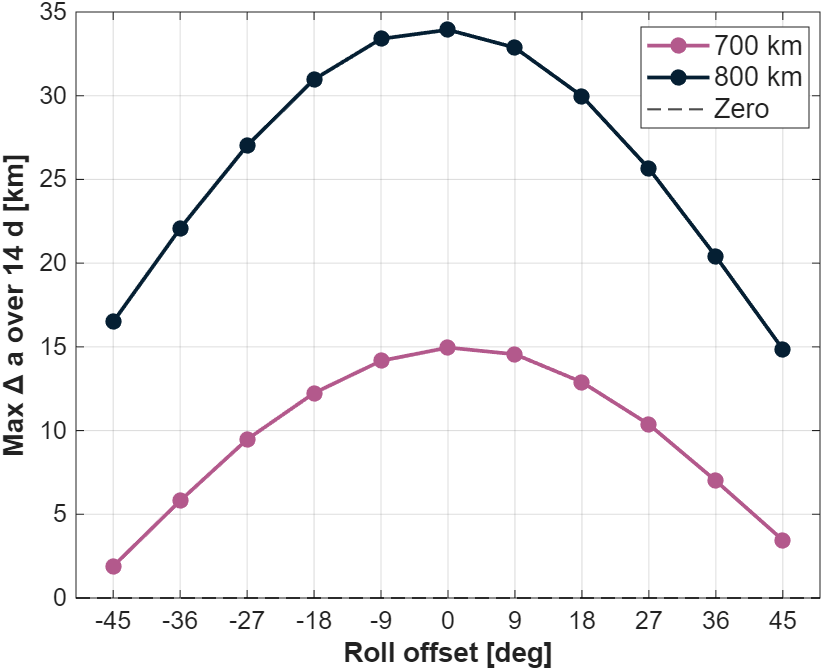
\includegraphics[width=0.92\linewidth]{Figures/fig6_w78.png}
   \captionof{figure}{Sensitivity of the \(14\)-day maximum semi-major-axis increase, \(\Delta a_{\max,14\mathrm{d}}\), to static roll offset about the gain-anchor attitude, shown for the same reference geometry propagated at \(700\,\mathrm{km}\) and \(800\,\mathrm{km}\). The common geometry is \(\Omega = 285.5^\circ\), LTDN \(=12.266176\,\mathrm{hr}\), pitch \(24.8^\circ\), zero roll offset, and \(A/m = 10\,\mathrm{m^2\,kg^{-1}}\). The response peaks at zero roll at both altitudes, but the bounded alignment envelope is substantially broader at \(800\,\mathrm{km}\).}
    \label{fig:roll_sensitivity_gain_anchor}
\end{center}

\vspace{0.5em}
\subsection{\textbf{Sensitivity to atmospheric density level}}

\noindent Figure~\ref{fig:density_sensitivity_gain_anchor} shows the effect of scaling the atmospheric density model by a constant multiplicative factor while holding the gain-anchor geometry fixed at both \(700\,\mathrm{km}\) and \(800\,\mathrm{km}\). At \(700\,\mathrm{km}\), the nominal atmosphere case (\(1\times\)) gives \(\Delta a_{\max,14\mathrm{d}} = 14.96\,\mathrm{km}\), which increases to \(28.59\,\mathrm{km}\) at \(0.5\times\) density and \(34.89\,\mathrm{km}\) at \(0.25\times\). Increasing density, however, suppresses the gain completely at this altitude: at \(2\times\) and \(4\times\) density, \(\Delta a_{\max,14\mathrm{d}} = 0\). At \(800\,\mathrm{km}\), by contrast, the same sweep remains positive throughout the full tested range, with \(33.94\,\mathrm{km}\) at nominal density, \(26.49\,\mathrm{km}\) at \(2\times\), and \(10.25\,\mathrm{km}\) even at \(4\times\) density.
\vspace{1em}
\par \noindent This sweep shows most clearly that drag is the dominant bounding mechanism, but it also shows that the location of the drag-limited boundary depends strongly on altitude. At \(700\,\mathrm{km}\), the short-horizon semi-major-axis increase exists only while the eclipse-biased SRP work surplus exceeds the accumulated drag losses; once the atmosphere is strengthened sufficiently, the drag penalty dominates from the outset and the semi-major axis never rises above its initial value within the \(14\)-day window. At \(800\,\mathrm{km}\), however, the same mechanism remains much more resilient: increased density degrades the gain substantially, but does not eliminate it across the tested range. The most defensible interpretation is therefore not that the regime is uniformly fragile, but that it is strongly altitude-dependent and can lie either near or well away from the drag-limited boundary depending on orbital height.

\begin{center}
     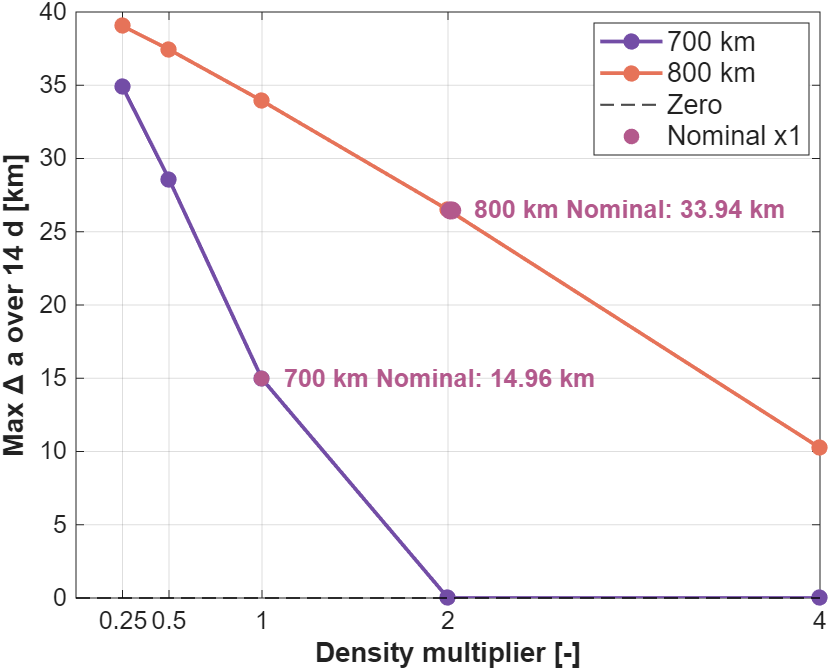
\includegraphics[width=0.92\linewidth]{Figures/fig7_w78.png}
   \captionof{figure}{Sensitivity of the \(14\)-day maximum semi-major-axis increase, \(\Delta a_{\max,14\mathrm{d}}\), to a multiplicative density scaling applied about the same gain-anchor geometry at \(700\,\mathrm{km}\) and \(800\,\mathrm{km}\). Reduced density strengthens the short-horizon gain at both altitudes. Increased density suppresses the \(700\,\mathrm{km}\) response completely by \(2\times\) nominal density, whereas the \(800\,\mathrm{km}\) case remains positive throughout the tested range, showing that the drag-limited boundary shifts substantially with altitude.}
    \label{fig:density_sensitivity_gain_anchor}
\end{center}


\vspace{0.5em}
\subsection{\textbf{Sensitivity to area-to-mass ratio}}

\noindent Figure~\ref{fig:amr_sensitivity_gain_anchor} shows the response to varying area-to-mass ratio while keeping the spacecraft mass fixed at \(10\,\mathrm{kg}\). The square sail side length is varied from \(5\) to \(15\,\mathrm{m}\), corresponding to \(A/m\) values from \(2.5\) to \(22.5\,\mathrm{m^2\,kg^{-1}}\). At \(700\,\mathrm{km}\), the response is non-monotonic. Starting from low \(A/m\), the maximum short-horizon gain rises from \(4.17\,\mathrm{km}\) at \(A/m=2.5\,\mathrm{m^2\,kg^{-1}}\) to the nominal \(14.96\,\mathrm{km}\) at \(A/m=10\,\mathrm{m^2\,kg^{-1}}\), then reaches a broad maximum of \(17.92\,\mathrm{km}\) at \(A/m=14.4\,\mathrm{m^2\,kg^{-1}}\), before declining slightly at larger sail sizes. At \(800\,\mathrm{km}\), by contrast, the response remains monotonic over the full sampled range, rising from \(8.54\,\mathrm{km}\) at \(A/m=2.5\,\mathrm{m^2\,kg^{-1}}\) to \(71.61\,\mathrm{km}\) at \(A/m=22.5\,\mathrm{m^2\,kg^{-1}}\), with no roll-over yet visible.
\vspace{1em}
\par \noindent The altitude split again changes the interpretation. At \(700\,\mathrm{km}\), the non-monotonicity shows that increasing sail size does not produce indefinite improvement: larger \(A/m\) strengthens SRP, but it also strengthens drag and modifies the coupled orbital response over the \(14\)-day window, producing a finite optimum and then a shallow plateau. At \(800\,\mathrm{km}\), however, the same drag-induced roll-over is pushed beyond the sampled range, so increasing \(A/m\) continues to improve the short-horizon gain throughout the tested envelope. The shared conclusion is that stronger SRP authority is beneficial, but the accessible benefit depends on how strongly drag competes over the observation window. Compared with the density sweep, the \(A/m\) response remains broad at both altitudes, but only the lower-altitude case shows a clear local optimum within the sampled range.

\begin{center}
    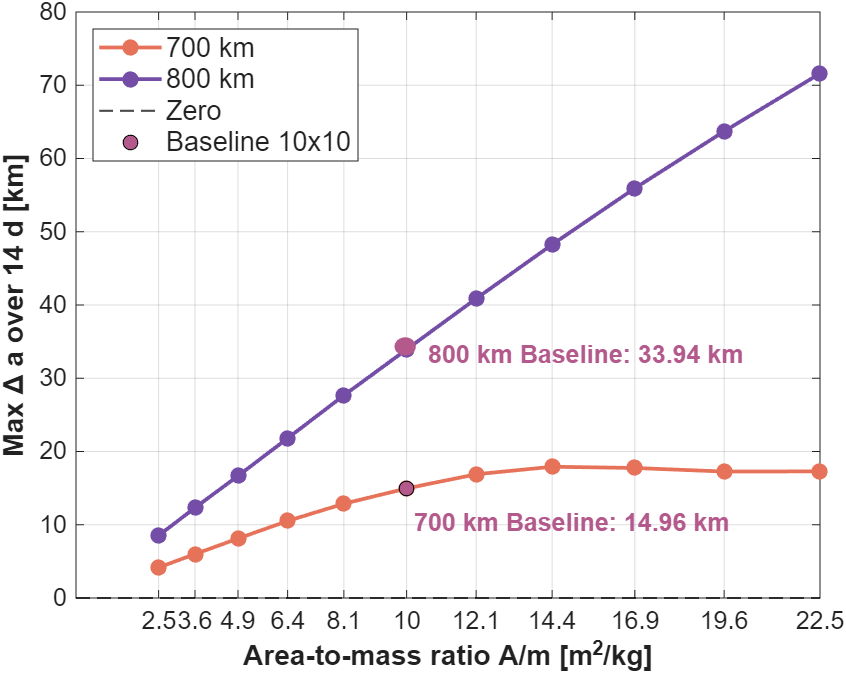
\includegraphics[width=1\linewidth]{Figures/fig8_w78.png}
    \captionof{figure}{Sensitivity of the \(14\)-day maximum semi-major-axis increase, \(\Delta a_{\max,14\mathrm{d}}\), to sail area-to-mass ratio for the gain-anchor case, with spacecraft mass held fixed at \(10\,\mathrm{kg}\), shown for the same reference geometry at \(700\,\mathrm{km}\) and \(800\,\mathrm{km}\). The \(700\,\mathrm{km}\) response is non-monotonic, with a broad optimum near \(A/m = 14.4\,\mathrm{m^2\,kg^{-1}}\), whereas the \(800\,\mathrm{km}\) response continues to increase across the full sampled range.}
    \label{fig:amr_sensitivity_gain_anchor}
\end{center}

\vspace{0.5em}
\subsection{\textbf{Interpretation of the sensitivity envelope}}

\noindent Taken together, the three sweeps support a restrained but more nuanced conclusion. The transient gain behaviour is not a numerically singular point: it persists over a finite neighborhood in roll and over a broad range of positive \(A/m\), and this admissible neighborhood expands significantly between \(700\,\mathrm{km}\) and \(800\,\mathrm{km}\). At the same time, the mechanism is still not a generally robust passive orbit-raising mode. Its existence remains contingent on favourable Sun-orbit-attitude phasing and on a drag environment weak enough for the eclipse-biased SRP work surplus to remain positive over the observation window.
\vspace{1em}
\par \noindent The most defensible statement is therefore that the gain occupies a bounded local envelope whose size depends materially on altitude. Roll sensitivity demonstrates finite but limited alignment tolerance at \(700\,\mathrm{km}\), but a substantially wider tolerance band at \(800\,\mathrm{km}\). Density sensitivity shows that drag remains the dominant bounding mechanism, while also showing that the regime can lie either close to or well away from the drag-dominated breakdown threshold depending on orbital height. Area-to-mass sensitivity shows that stronger SRP authority improves the short-horizon gain broadly, but that the onset of diminishing returns is itself altitude-dependent and is shifted to larger \(A/m\) at higher altitude. These results are consistent with the broader thesis of the paper: the mechanism is real and physically interpretable, but it is geometry-bounded, alignment-sensitive, and ultimately limited by the coupled drag and orbital-distortion effects that later drive the long-horizon transition from transient gain to decay.

\FloatBarrier